\documentclass{article}

% set font encoding for PDFLaTeX, XeLaTeX, or LuaTeX
\usepackage{ifxetex,ifluatex}
\if\ifxetex T\else\ifluatex T\else F\fi\fi T%
  \usepackage{fontspec}
\else
  \usepackage[T1]{fontenc}
  \usepackage[utf8]{inputenc}
  \usepackage{lmodern}
\fi

\setlength{\parindent}{0pt}


\usepackage[catalan,english,spanish]{babel}
\usepackage{hyperref}
\usepackage{color}
\usepackage{amsmath}
\usepackage{graphicx}
\usepackage{amsfonts}
\usepackage{svg}
\usepackage{comment}
%\usepackage{parskip}


\newcommand{\HRule}{\rule{\linewidth}{0.5mm}}


\title{Neuroevolución de topologías aumentadas}
\author{Aurelio Losquiño Muñoz}

% Enable SageTeX to run SageMath code right inside this LaTeX file.
% http://doc.sagemath.org/html/en/tutorial/sagetex.html
% \usepackage{sagetex}

% Enable PythonTeX to run Python – https://ctan.org/pkg/pythontex
% \usepackage{pythontex}

\begin{document}
\begin{titlepage}
\centering
\textsc{Universidad Autónoma de Barcelona}\\
\textsc{Trabajo de fin de grado}\\[1cm]
\HRule \\[0.4cm]
{ \huge \bfseries Neuroevolución de topologías aumentadas}\\[0.4cm]
\HRule \\[1.5cm]
\textsc{\large Aurelio Losquiño Muñoz}\\[0.5cm]
\textsc{Junio de 2020}
\end{titlepage}

\begin{abstract}
\setlength{\parindent}{0pt}
\noindent Durante los últimos años, la inteligencia artificial ha tomado un papel clave en el desarrollo de la humanidad. Haciendo uso de métodos de aprendizaje automático, se ha conseguido diseñar coches autodirigidos, robots capaces de realizar volteretas y programas que juegan a ajedrez a un nivel sobrehumano.\\

En este trabajo se estudiará a fondo el algoritmo genético NEAT y se implementará en python3 a partir del paper del algoritmo. Con ello, se consigue dominar un juego estilo \textit{Flappybird} y otros entornos de openAI gym como el CartPole-v0 y el MountainCar-v0. Por último, se tratará de crear una inteligencia artificial que juegue al cuatro en raya.

\end{abstract}
\selectlanguage{catalan}
\begin{abstract}
\setlength{\parindent}{0pt}
\noindent Durant els últims anys, la intel·ligència artificial ha pres un paper clau en el desenvolupament de la humanitat. Fent ús de mètodes d'aprenentatge automàtic, s'ha aconseguit dissenyar cotxes autodirigits, robots capaços de realitzar tombarelles i programes que juguen a escacs a un nivell sobrehumà. \\

En aquest treball s'estudiarà a fons l'algoritme genètic NEAT i s'implementarà en python3 a partir del paper de l'algoritme. Amb això, s'aconsegueix dominar un joc de l'estil \textit{Flappybird} i altres entorns d'openAI gym com el CartPole-v0 i el MountainCar-v0. Finalment, es tractarà de crear una intel·ligència artificial que jugui al quatre en ratlla.
\end{abstract}
\selectlanguage{english}

\begin{abstract}
\setlength{\parindent}{0pt}
\noindent During the past few years, artificial intelligence has played a key role in the development of humanity. Using machine learning methods, it has been possible to design self-driving cars, robots able to backfliping and programs that play chess at a superhuman level.\\

In this work, the NEAT genetic algorithm will be deeply studied and it will be implemented in python3 from the algorithm paper. With this, it is possible to master a game similar to \textit{Flappybird} and other openAI gym environments such as CartPole-v0 and MountainCar-v0. Finally, the goal will be creating an artificial intelligence that plays connect four.
\end{abstract}
\selectlanguage{spanish}

\newpage
\tableofcontents
\newpage
\section{Introducción}

La inteligencia artificial ha cambiado nuestro presente y cambiará el futuro. Son muchos los avances en la sociedad gracias a las inteligencias artificiales, desde el reconocimiento facial o de voz hasta la conducción automovilística automática. El potencial de la inteligencia artificial es inimaginable y la importancia de comprenderla va más allá del puro interés académico. Uno siempre lleva consigo un dispositivo móvil que está constantemente transmitiendo información personal. ¿Hasta qué punto podrían las empresas aseguradoras recoger todos esos datos para entrenar un modelo que determine que tan mal ha envejecido una persona?\\

En este trabajo se pretende estudiar e implementar el algoritmo Neuroevolución de topologías aumentadas (NEAT) en python3 de manera que sea totalmente funcional. Se evaluará el algoritmo en distintos entornos bien conocidos dentro del mundo del aprendizaje por refuerzo como son por ejemplo los de plataforma \textit{gym} de OpenAI entre otros.\\

Para la implementación del NEAT se revisarán los papers de los autores sobre él. Además se comparará con otras implementaciones ya hechas con tal de garantizar el buen funcionamiento y rendimiento de la implementación. Por último se programarán algunos entornos donde probar el algoritmo y un programa de visualización gráfica.\\

Este trabajo comienza dando una breve noción sobre algunos de los conceptos básicos y necesarios para entender el algoritmo. Posteriormente se estudia como funciona el algoritmo NEAT y por último se muestran una serie de resultados obtenidos con la implementación realizada.\\


\begin{comment}

Hay que tener en cuenta que cada vez que se resuelve en internet un \textit{captcha} o se sube a una red social una foto se están donando posibles datos de entrenamiento para una inteligencia artificial.\\
A principios del año 2018 se hizo viral el hecho de publicar una foto comparativa entre una fotografía actual y una de hace diez años. 

Uno siempre lleva consigo un dispositivo móvil que está constantemente haciendo uso de ella. De hecho cuando la empresa Google nos hace resolver un \textit{captcha} para comprobar que no somos un sotfware, usa ese captcha para entrenar a sus modelos de reconocimiento de imágenes.\\

\url{https://www.youtube.com/watch?v=Wi5Tq1Q_nHk}.\\
tema- no poner: el tfg trata sobre IA. mejor poner La inteligencia artificial es super importante hoy en dia por ejemplo para conducir automaticamente.  las IAS pueden desarrollar estrategias sobrehumanas en juegos y podria ser a plicablea ...justificar el interes mundial del tema.\\

antecedentes historicos??


\begin{comment}
objetivos- objetivos generales y especificos. delimitar claramente los objetivos, dejar claro el alcance del trabajo, a donde queremos llegar  y a donde no. es el momento de advertir sobre temas que no vamos a tocary si es necesario justificar el motivo por el cual no se estudia eso.\\

metodologia- se implementara en python3 a traves del paper

estructura- esxplicar la estructura del trabajo: eeste trabajo comienzo repasando unos conceptos previos para pode tratar el tema principal\\
\end{comment}

\section{Conceptos previos}

\subsection{Red neuronal}
Intuitivamente una red neuronal artificial es un conjunto de unidades que se conocen como neuronas (o nodos) conectadas entre sí. Las redes neuronales artificiales reciben este nombre debido a la semejanza que hay entre su representación gráfica y una red neuronal de un cerebro biológico.\\

\begin{figure}[htbp]
% http://alexlenail.me/NN-SVG/index.html
\centering
\includegraphics[trim={24cm 13cm 0 6cm},clip,width=20cm]{nn.pdf}
% trim={<left> <lower> <right> <upper>}
\caption{Representación gráfica de una red neuronal}
\end{figure}
Formalmente una red neuronal es un modelo estadístico que forma parte del deeplearning. El deeplearning (o también conocido como aprendizaje profundo) es una rama específica del aprendizaje automático (o machine learning).\\


Sea $c$ el número de capas de una red neuronal con $n_k$, $1\leq k\leq c$ neuronas en cada capa. Cada neurona de la red estará conectada con cada una de las neuronas de sus capas adyacentes. Sea $a_i^{(k)}$ la $i$-ésima neurona $1\leq i\leq n_k$ de la capa $k$, $1\leq k\leq c$. Cada neurona contendrá un umbral de activación (también conocido como bias o sesgo), que será un número real y lo denotaremos por $u_i^{(k)} $. La conexión de la $i$-ésima neurona de la capa $k$ con la $j$-ésima neurona de la capa $k+1$ la denotaremos por $\omega_{ji}^{(k)} $. Tanto los pesos como los umbrales se inicializan de manera aleatoria. Cada neurona que no se encuentre en la primera capa posee lo que se conoce como una función de activación. Las más usadas son la sigmoide
$$\sigma(x)=\frac{1}{1+e^{-x}} $$
y la Relu
$$\text{Relu}(x)=\max(0,x) $$
La función de activación suele ser común por todas las neuronas de la red, aunque es posible que esto no sea así.\\

La red neuronal tomará como input un vector real de longitud $n_1$. En concreto la componente $i$-ésima del vector será el input y output de la neurona $a_i^{(1)}$.\\
El input de la neurona $a_i^{(k+1)} $ será
$$z_i^{(k)}=\sum_{j=1}^{n_k} \omega_{ji}^{(k)} a_j^{(k)}+u_j^{(k)} $$
y su output será
$$a_i^{(k+1)}=f(z_i^{(k)}) $$
donde $f$ es su función de activación.

\subsection{Bondades de las redes neuronales}
% https://towardsdatascience.com/history-of-the-first-ai-winter-6f8c2186f80b
En el 1969 se vio que los modelos que se podían lograr con redes neuronales de dos capas únicamente podían resolver problemas de separación lineal. En particular red neuronal de este tipo no podía imitar una puerta lógica XOR \cite{HistoryofthefirstAIWinterTowardsDataScience-2020-06-19}.\\

\begin{figure}[htbp]
\centering
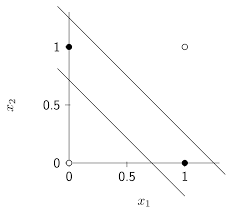
\includegraphics[width=4cm]{XOR.png}
\caption{Visualizacación de la separación no lineal de la puerta XOR}
%foto sacada de este enlace 
% https://encrypted-tbn0.gstatic.com/images?q=tbn%3AANd9GcReKA3PNHEG6uEIRj97rpD1UHESUsqq2OzXvIzWzt7K-YSf7WPv&usqp=CAU
\end{figure}
Se sabía que una red neuronal más compleja (con más de dos capas) sí que podía hacer esa tarea. Sin embargo a la práctica no era posible, ya que el hardware era poco potente y los métodos que se conocían para entrenar las redes eran lentos.\\
Hoy en día esto ya no es un problema debido a que posteriormente se inventó el algoritmo conocido como backpropagation que junto con el descenso del gradiente permiten entrenar redes neuronales muy complejas a una velocidad muy alta.\\

% https://www.youtube.com/watch?v=y7NdSrkrwqI
% http://neuralnetworksanddeeplearning.com/chap1.html
En la figura \ref{fig:red_nand} se muestra la representación de una red neuronal que reproduce una puerta lógica NAND.
\begin{figure}[htbp]
\centering
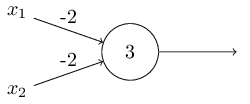
\includegraphics[width=4cm]{NAND.png}
\caption{Red neuronal modelizando una puerta NAND}
\label{fig:red_nand}
\end{figure}
Esta es una red con dos capas: la primera contiene dos neuronas y la segunda solo una con un umbral igual a $3$. Además observamos que los pesos de las dos únicas conexiones son iguales a $-2$. En este caso la función de activación de la neurona de la segunda capa es 
$$f(x)=\begin{cases}
1 \text{ si } x>0\\
0 \text{ si } x\leq 0\\
\end{cases}.$$

En efecto, como se puede ver en la figura \ref{fig:tabla_verdad}, la red reproduce la tabla de la verdad de la puerta lógica NAND.\\
\begin{figure}[htbp]
\centering
\begin{tabular}{ |c|c|c| } 
 $x_1$ & $x_2$ & output \\ 
 \hline
 0 & 0 & $f(0\cdot (-2)+0\cdot (-2)+3)=f(3)=1$ \\ 
 0 & 1 & $f(0\cdot (-2)+1\cdot (-2)+3)=f(1)=1$ \\ 
 1 & 0 & $f(1\cdot (-2)+0\cdot (-2)+3)=f(1)=1$ \\ 
 1 & 1 & $f(1\cdot (-2)+1\cdot (-2)+3)=f(-1)=0$ 
\end{tabular}
\caption{Tabla de la verdad de la red neuronal representada en la figura \ref{fig:red_nand}}
\label{fig:tabla_verdad}
\end{figure}

Las puertas NAND son universales para la computación, es decir, se puede conseguir cualquier puerta lógica como combinaciones de estas. Como consecuencia tenemos que una red neuronal suficientemente compleja podría reproducir un modelo tan complejo como queramos, con la ventaja de que este modelo se creará solo mediante el ajuste de pesos y umbrales \cite{Neuralnetworksanddeeplearning-2019-12-27}.\\

Hay que tener en cuenta que un ligero cambio en un peso podría cambiar por completo el comportamiento del modelo. Para evitarlo se suele usar como función de activación la función sigmoide, que se puede ver como una versión diferenciable de la función de activación anterior. Esto asegura que una pequeña variación en los pesos y/o umbrales resulte en una pequeña variación en el output del modelo.\\

Hay que destacar que el teorema de aproximación universal establece que una red neuronal de tres capas con función de activación la sigmoide puede aproximar arbitrariamente una función continua en cualquier compacto de $\mathbb{R}^n $ \cite{UniversalapproximationtheoremWikipedia-2020-06-19}.
% Es posible que en lugar de 3 capas sean 2. ver link:
% https://en.wikipedia.org/wiki/Universal_approximation_theorem

\subsection{Aprendizaje por refuerzo}
Uno de los logros de las redes neuronales ha sido la clasificación o reconocimiento de imágenes, como por ejemplo el reconocimiento de dígitos escritos a mano. Para atacar este tipo de problemas, se necesitan grandes datos de entrenamiento, es decir un conjunto de ejemplos clasificados correctamente. Como hemos dicho antes, los pesos y los umbrales serán inicializados de manera aleatoria. Con los datos de entrenamiento y mediante un algoritmo conocido como backpropagation, junto con el método del descenso del gradiente, se consiguen ajustar los pesos para conseguir un buen modelo. Usar datos de entrenamiento ya resueltos para entrenar el modelo es una técnica del machine learning conocida como aprendizaje supervisado.\\

En este trabajo se estudia un método de lo que se conoce como aprendizaje por refuerzo (o reinforcement learning). La diferencia fundamental entre el aprendizaje supervisado y el aprendizaje por refuerzo es que en el aprendizaje supervisado se necesita conocer el output deseado para cualquier input. El problema viene cuando queremos hacer un programa informático que dé una respuesta a un problema que nosotros no sabemos resolver, como por ejemplo, dada una posición de ajedrez determinar cuál es el mejor movimiento.\\

El aprendizaje por refuerzo es un conjunto de técnicas que sirven para entrenar un modelo mediante lo que se conocen como recompensas o castigos. Por lo tanto para entrenar un modelo con estas técnicas no es necesario saber cual es la respuesta óptima pero si es necesario saber distinguir si la respuesta es mejor a otra o no.

\subsection{Algoritmos genéticos}
\subsubsection{Conceptos generales}
Los algoritmos genéticos podemos considerarlos como una técnica para el aprendizaje por refuerzo. La idea de estos algoritmos es tener una población de agentes, dejar que estos tomen decisiones en función de sus criterios propios y seguidamente asignarles un fitness. El fitness es un valor numérico que debe representar lo bien que ha hecho el agente la tarea a resolver. Finalmente, a cada agente se le asigna una probabilidad de reproducirse en función de su fitness y, tras el cruce con otro individuo y una posible mutación, se crea una nueva generación de agentes. La idea es que el cruce entre los agentes produzca un nuevo agente que de alguna manera herede las bondades de sus antecesores. Por lo tanto con el paso de las generaciones, los agentes tendrán en mejor desempeño para realizar la tarea (tendrán mayor fitness).\\

Los agentes o individuos de la población serán escogidos acorde con el problema a resolver. Del mismo modo, habrá que diseñar un algoritmo que dados dos individuos genere un descendiente potencialmente mejor a sus predecesores.\\

Es posible que al crear una nueva generación, esta sea peor que su predecesora. Para evitarlo, se usa una técnica conocida como elitismo. Esta técnica consiste en añadir a la nueva generación una copia exacta del mejor de la generación anterior. De este modo se asegura el no empeoramiento generación tras generación.\\

Uno de los puntos clave de los algoritmos genéticos es la diversidad dentro de la población. Si nuestra población inicial es muy pequeña o no está distribuida de manera uniforme, se necesitarán muchas generaciones para que, a través de la mutación, se genere la diversidad necesaria. También es posible que mediante el cruce se pierda diversidad genética. Por ello, se asigna una pequeña probabilidad al hecho de que un nuevo agente sea mutado.\\

A menudo suele ocurrir que empieza a haber un individuo dominante y por lo tanto la siguiente generación es, en mayor parte, descendiente de él. Esto en general hace que toda la población converja hacia un mismo agente, lo que significa que se alcanzará un máximo local en la función fitness. Un método para tratar de evitar la convergencia hacia un máximo local es lo que se conoce como proteger la innovación mediante la especiación.
Esta técnica consiste en separar los individuos en especies, de manera que los individuos se reproduzcan y compitan únicamente con los de su especie.

\subsubsection{Generación de frases}
Supongamos que nuestro objetivo es hacer un programa que escriba en el ordenador la palabra \textit{matemáticas}. Obviamente esto no es un desafío real, pero es un buen ejemplo para comprender la esencia de los algoritmos genéticos.\\
En este caso los individuos de nuestra población serán palabras de 11 caracteres que, inicialmente, serán generadas de manera totalmente aleatoria.\\

El fitness de un individuo (palabra) será el número de caracteres correctos (misma posición y carácter que la palabra objetivo \textit{matemáticas}). A continuación asignaremos a cada individuo una probabilidad de ser escogido frente al resto para reproducirse proporcional a su fitness.\\

Dados dos individuos podemos generar un descendiente escogiendo los caracteres correctos de cada uno. Si un carácter no es correcto en ninguno de los dos, escogeremos de manera equiprobable entre los dos de sus antecesores en esa misma posición.\\

A continuación podemos imponer que uno de cada cien descendientes padezca una mutación. En este caso una mutación podría ser simplemente escoger un carácter al azar de la palabra y cambiarlo por otro carácter al azar del abecedario. Observamos que en este caso la mutación favorece a la creación de diversidad. En efecto, podría ser que ninguna de nuestras palabras iniciales tuviera como primera letra la $m$ y como consecuencia (por como hemos definido el cruce entre individuos) el objetivo nunca se podría alcanzar.


\section{Neat}

% enlace al paper original
% http://citeseerx.ist.psu.edu/viewdoc/download?doi=10.1.1.28.5457&rep=rep1&type=pdf

El algoritmo Neuroevolución de topologías aumentadas (NEAT) es un algoritmo genético para evolucionar redes neuronales desarrollado por Kenneth O. Stanley y Risto Miikkulainen en el año 2001 \cite{EvolvingNeuralNetworksthroughTopologies}\cite{EfficientEvolutionofNeuralNetworkTopologies}.\\

La idea clave del algoritmo es empezar con una población de redes neuronales lo más pequeñas posible e ir aumentando su topología (forma) progresivamente mediante el cruce entre ellas y/o la mutación. Intentar entrenar una red neuronal con una topología fijada desde un inicio con algoritmos genéticos sería demasiado costoso computacionalmente. NEAT da la posibilidad de que el modelo se haga cada vez más complejo y preciso con el paso de las generaciones, fortaleciendo, si cabe, la analogía con la evolución biológica.\\

Una ventaja adicional de evolucionar progresivamente la topología es que la red crecerá solo cuando sea necesario, garantizando así redes prácticamente minimales.\\

Frecuentemente, añadir nueva estructura a una red causa un empeoramiento en su fitness. Por ejemplo, añadir un nuevo nodo en medio de una conexión introduce una nolinealidad donde antes no la había. Lo mismo sucede si se añade una nueva conexión: se necesitarán varias generaciones para optimizar sus pesos.\\

Por lo tanto, la bajada en el desempeño de las redes con estructura innovadora provocaría una disminución en su fitness y como consecuencia que la innovación no se propague hacia las siguientes generaciones. El algoritmo NEAT propone un método para separar las redes en especies, de manera que las redes con nueva estructura no compitan directamente con toda la población.\\
\subsection{Inicialización}
Inicialmente las redes tendrán únicamente dos capas de neuronas: la del input y la del output. La cantidad de nodos en dichas capas vendrá determinada por las necesidades de la tarea a realizar. Además no tendrán ninguna conexión, estas deberán aparecer en futuras generaciones mediante la mutación.\\

El algoritmo NEAT asigna a cada nodo y conexión lo que denominan el número de innovación. Los números de innovación son marcadores históricos que identifican el origen de cada nodo/conexión. Estos números de innovación son globales y comunes para todas las redes, de manera que si dos redes poseen el mismo nodo/conexión entonces estos debe tener el mismo número de innovación. Los números de innovación se van asignando progresivamente cada vez que una innovación aparece a través de la mutación. De este modo, los números de innovación servirán para facilitar la comparación topológica entre dos redes. En la figura \ref{fig:inn} se muestra una posible mapeado de los números de innovación.

\begin{figure}[htbp]
\centering
\includegraphics[width=13cm]{innovation_number.png}
\caption{Codificación de los genes (nodos y conexiones) de una red neuronal con sus respectivos número de innovación.}
\label{fig:inn}
\end{figure}



\subsection{Mutación}
La mutación en NEAT puede ser de varias maneras. Hay dos mutaciones principales, que añaden estructura nueva a la red. La primera consiste en reemplazar (desactivar) una conexión ya existente por una estructura conexión-nodo-conexión. En este caso la conexión que va hacia el nuevo nodo recibirá un peso de 1 y la conexión con origen el nuevo nodo recibirá el mismo peso que tenía la antigua conexión. La segunda mutación consiste en añadir una nueva conexión con un peso aleatorio entre dos nodos no conectados que no estén en la misma capa. En la figura \ref{fig:mutacion} se muestra un ejemplo de cada una de estas mutaciones. Nótese el uso del número de innovación para las nuevas estructuras.\\

\begin{figure}[htbp]
\centering
\includegraphics[width=13cm]{mutation.jpg}
\caption{Visualización de la mutación de una red en NEAT}
\label{fig:mutacion}
\end{figure}

Como se puede ver, cada rectángulo corresponde a una conexión y en su posición más alta se indica su número de innovación. Obsérvese que, siguiendo con la notación del ejemplo, si una red cualquiera padece una mutación en la que se le añade una conexión, que conecta los nodos con número de innovación 3 y 5, esta deberá tener como número de innovación 7. Por otro lado, siempre que la conexión con número de innovación 3 sea reemplazada por un nodo y sus dos correspondientes conexiones, el nodo deberá tener un 6 como número de innovación y las conexiones 8 y 9 respectivamente.\\

Hay otro tipo de mutaciones secundarias que no añaden nueva estructura a la red. Estas son:
\begin{enumerate}
\item Escoger aleatoriamente una conexión ya existente y cambiarle su peso.
\item Escoger aleatoriamente una conexión y modificarle ligeramente su peso.
\item Escoger aleatoriamente una conexión y activar (o desactivar) la conexión.
\end{enumerate}
Es posible hacer muchas variaciones en este tipo de mutaciones, ya sea escogiendo una distribución probabilística determinada y/o fijando límites a los pesos que se pueden asignar.

\subsection{Crossover}
El punto clave del algoritmo NEAT es el cruce (o crossover) entre dos redes y es lo que, en parte, justifica la asignación de los números de innovación. En la figura \ref{fig:crossover} se muestra un esquema de la idea del crossover.\\

\begin{figure}[htbp]
\centering
\includegraphics[trim={0 0 0 0},clip,width=13cm]{crossover.png}
\caption{Visualización del crossover en NEAT}
\label{fig:crossover}
\end{figure}

Como se puede observar, dadas dos redes se comparan los números de innovación de las conexiones de cada una. Si una conexión es común en ambas redes, el descendiente heredará la conexión del padre con mayor fitness. Si hay una conexión que no es compartida por ambas redes entonces esta será heredada únicamente si dicha conexión pertenece al padre más fit. Nótese que en el ejemplo gráfico de la figura \ref{fig:crossover} se asumen ambas redes de igual fitness y por lo tanto todas las conexiones son transferidas al sucesor.\\

Este método resulta ser computacionalmente rapidísimo. Se ahorra mucho tiempo al no tener que hacer una búsqueda exhaustiva topológica de los grafos que forman la red, a cambio de reservar una cantidad minúscula de memoria para los números de innovación.\\

Nótese que en la figura \ref{fig:crossover} se le dice conexión disjunta a las que su número de innovación está comprendido entre los números de innovación de las conexiones de una segunda red. Similarmente, se conoce como conexión de exceso a las que su número de innovación es mayor al de las conexiones de una segunda red.

\subsection{Especiación}
\label{especiacion}
Como se ha comentado anteriormente, la especiación es clave para garantizar la supervivencia de la innovación. A menudo cuando la innovación aparece a través dela mutación, este produce un descenso en el fitness de la red. Como consecuencia la innovación no tiene muchas posibilidades de pasar a la siguiente generación. Separar los individuos de la población en distintas especies de acuerdo con su topología permite que estas compitan únicamente entre sus compañeros. Esto permite empezar con redes mínimamente pequeñas debido a que se garantiza el aumento adecuado de la complejidad del modelo. Con todo esto no solo se ahorra mucho tiempo de computación sino que también se consiguen modelos lo más sencillos posible.\\

El problema de separar a las redes en distintas especies parece un problema de coincidencia topológica. Sin embargo, de nuevo los números de innovación convierten este problema en algo mucho más sencillo.\\
%\textcolor{red}{competing conventions: The competing conventions problem arises when there is more than one way of representing information in a phenotype. For example, if a genome contains neurons A, B and C and is represented by [A B C], if this genome is crossed with an identical genome (in terms of functionality) but ordered [C B A] crossover will yield children that are missing information ([A B A] or [C B C]), in fact 1/3 of the information has been lost in this example. NEAT solves this problem by tracking the history of genes}\\

Dadas dos redes $i,j$, sea $E$ la cantidad de conexiones de exceso, $D$ la cantidad de genes disjuntos y $\overline{W}$ la media de los pesos de las conexiones que coinciden en ambas redes. El algoritmo NEAT propone la siguiente medición para la distancia genética entre dos redes:
$$\delta(i,j)=\frac{c_1E}{N}+\frac{c_2D}{N}+c_3\overline{W} $$

donde los coeficientes $c_1,c_2,c_2 $ son pesos que se podrán escoger cuando se use el algoritmo. $N$ es la mayor de las cantidades de conexiónes de cada red, aunque si $N<20 $ se puede tomar $N=1$. Esta fórmula nos permite clasificar a los individuos en diferentes especies en función de su distancia genética $\delta$ cuando esta supere un cierto umbral $\delta_u$.\\

Con tal de proteger a las nuevas especies, NEAT usa un método conocido como \textit{fitness sharing}. Este método consiste en \textit{compartir} el fitness de los individuos entre los de su especie. Si $f_i$ es el fitness del $i$-ésimo individuos entonces su fitness ajustado $f_i'$ pasa a tener el valor de 
$$f_i'=\frac{f_i}{\sum_{j=1}^n \text{sh}(\delta(i,j))} $$
donde sh es conocida como la share function y esta es una función a determinar. En el algoritmo NEAT, la función sh toma el valor 1 si $\delta(i,j)<\delta_u $ y 0 en caso contrario.\\

\subsection{Nueva generación}
El método para crear una nueva generación a partir de la anterior es el siguiente:
\begin{enumerate}
\item Se mantiene la lista de especies de la generación anterior. Al inicio de una nueva generación, a cada especie se le asigna un representante aleatorio de entre sus miembros. A continuación, los no representantes de alguna especie se asignan a la primera especie tal que su distancia genética $\delta$ con su representante sea menor a un cierto umbral $\delta_u$. En el caso que un individuo no sea compatible con ninguna especie, una nueva especie será creada con este individuo como representante.
\item Se ajusta el fitness de cada individuo tal y como se ha descrito en la sección \ref{especiacion}.
\item Se elimina el $m\%$ menos fit de la población, donde $m$ es un paramétro a escoger. Tras la eliminación, si alguna especie resulta tener un individuo (o ninguno) esta especie será extinguida.
\item A cada especie se le asigna una probabilidad parar cruzar a dos individuos suyos proporcional a la suma de los fitness ajustados de sus integrantes. A su vez, dentro de cada especie cada individuo tiene una probabilidad de reproducirse proporcional su propio fitness.\\

Mientras el número de individuos actual no sea igual al número de individuos inicial, se van escogiendo especies para el cruce. Cuando se escoge una especie para la reproducción, se escogen dos individuos de esta y se crea su descendiente. El descendiente padecerá una mutación con una cierta probabilidad a determinar (normalmente en torno al $1\%$) y será asignado a la misma especie que sus progenitores con un fitness de 0.
\end{enumerate}

\section{Implementación}
He programado el algoritmo NEAT en python3 usando únicamente la librería estándar y numpy. A continuación se muestra una lista de los hiper-parámetros que se pueden editar en mi implementación personal y sus respectivos valores por defecto.
\begin{itemize}
\item Número total de individuos en la población. Esta cantidad permanecerá fija durante todo el proceso: se repoblará con exactamente la cantidad de muertos. (100)
\item Número de nodos de input/output. Estos parámetros no tienen valores por defecto, pues deben ser determinados específicamente para cada caso.
\item Función de activación de las neuronas entre sigmoide o RELU. (RELU)
\item Coeficientes para el cálculo de la distancia genética y el umbral genético $(c_1,c_2,c_3,\delta_u) $. $(1,1,1,4) $
\item El porcentaje $m\%$ de muertes al final de cada generación. $(50\%) $
\item Probabilidad de mutar un nuevo nodo. (0.05)
\item Probabilidad de mutar una nueva conexión. (0.05)
\item Probabilidad de mutar un ajuste de peso. (0.5)
\item Probabilidad de mutar un cambio de peso. (0.2)
\item Probabilidad de mutar activación/inhibición de conexión. (0.1)
\item Rango de la distribución uniforme para el ajuste de peso. (1)
\item Rango de la distribución uniforme para el cambio de peso. (0.3)
\item Pese a no ser un hiper-parámetro como tal, se deberá escoger una función para determinar el fitness de las redes.

\end{itemize}
Nótese que una elección adecuada de estos parámetros puede acelerar el desarrollo del algoritmo. Por contra, es posible que una mala elección haga que el algoritmo jamás logre evolucionar una red de manera satisfactoria.\\

Durante la implementación se ha comparado con códigos de terceros con tal de asegurarse que la implementación sea lo más eficiente posible computacionalmente hablando: el código ha sido optimizado tanto en cuanto a tiempo de ejecución como a memoria RAM requerida. Como se ha podido comprobar, en los papers del NEAT hay puntos donde no se da información suficientemente precisa. Como consecuencia, el programador debe decidir como lidiar con algunas situaciones no contempladas en los papers.\\

%Para ver más detalles sobre la código véase el Anexo 1. G anexo o anexo 1?\\

%\textcolor{red}{Poner foto de la terminal del neat.\\Adicionalmente he decidido crear otro programa para poder visualizar mejor las redes.}


\section{Resultados}
En general el aprendizaje por refuerzo tiene como objetivo desarrollar algoritmos para controlar algún tipo de maquinaria. Por ejemplo se podría conseguir un algoritmo que permita a un robot caminar o incluso correr sobre sus dos piernas. Para entrenar estos algoritmos se suelen programar entornos en los que se simulen eventos que podrían darse en la realidad. Del mismo modo que los simuladores aéreos permiten entrenarse a los pilotos de avión, estos entornos hacen que la inteligencia artificial aprenda sin producir gastos económicos con sus tempranos errores. En este caso, el robot caería al suelo únicamente dentro de un entorno virtual y no necesitaría ser reparado tras cada fallo del algoritmo.\\

En esta sección se pondrá a prueba la implementación del NEAT en varios entornos comunes para ver su rendimiento. En cada uno de los entornos se establece cuando se considera superado. En cada entorno, el usuario debe decidir que datos tomar para usarlos como input a las redes y, similarmente, el número de acciones posibles determinará el número de outputs de la red. Alimentar a la red con muchas variables hará que estas sean más grandes pero también tendrán más información para su toma de decisiones. Saber identificar los datos importantes también es un factor clave y, por suerte, a menudo esto suele ser fácil.\\

Para cada entorno se contabilizarán el número medio de generaciones necesarios para llegar a una solución (si es que se consigue) y cuales son los hiper-parámetros óptimos para ello. A su vez también se verá cual es la red más pequeña encontrada como solución.
\subsection{Flappy bird}
El \textit{Flappy bird} es un conocido videojuego para móvil que se viralizó hace unos pocos años. Es un juego extremadamente sencillo y con el que el algoritmo NEAT ha ganado mucha fama a través de internet.\\

El juego original consiste en decidir cuando un pájaro debe darse un pequeño impulso hacia arriba con tal de no chocarse con unas tuberías que se encuentran por el camino. En este caso se ha programado en python3 un entorno en el que únicamente se han reproducido las mecánicas del juego (sin animaciones ni dibujos).\\
\begin{figure}[htbp]
\centergin
\includegraphics[width=10cm]{FlappyBird.png}
\caption{Captura de pantalla del entorno Flappy Bird}
\end{figure}



Nótese que si nuestro objetivo fuera hacer un bot inmortal para este juego, desde luego usar estos métodos de inteligencia artificial no serían necesarios. Sin embargo, es un muy buen primer test para nuestra implementación del NEAT.\\

Para este juego las redes neuronales tomarán como input la posición del pájaro y la posición de la columna más cercana. Parece razonable pensar que es suficiente con conocer la posición relativa a la tubería más cercana y a su vez esto nos permitirá mantener lo más pequeña posible las redes. Más precisamente la red tendrá 3 inputs. El primero será la distancia vertical entre el pájaro y el límite superior. El segundo será la distancia vertical entre la esquina superior izquierda de la parte inferior de la tubería. Por último, el input del tercer nodo será la distancia horizontal entre el pájaro y la siguiente columna más cercana. Además estos tres inputs serán normalizados, es decir, se reescalan con tal de que estén compredidos en el intervalo $[0,1]$. Este último detalle técnico es muy común en las redes neuronales y favorece a la regularidad del proceso.\\

Puesto que la única acción existente en el juego es saltar (o no hacer nada), la red tendrá un único output. Usaremos el siguiente criterio para interpretar el output de la red: Si el output es mayor a $0.5$ entonces saltará, en caso contrario no hará nada (se dejará caer).\\

El fitness asignado a cada red será el número de obstáculos sorteados dividido por el número de nodos de la red. De este modo estaremos premiando a los pájaros que lleguen más lejos y castigando el crecimiento de las redes. El hecho de que sea un juego tan simple hace pensar que no será un necesario un modelo muy complejo para dominarlo y por lo tanto una red pequeña será suficiente. \\

Los hiper-parámetros escogidos para este caso serán:
\begin{itemize}
\item Probabilidad de mutar nuevo nodo: 0.001
\item probabilidad de mutar nueva conexión: 0.7
\item probabilidad de mutar ajuste de peso: 0.3
\item probabilidad de mutar nuevo peso: 0.8
\item Probabilidad de activar conexión: 0.3
\item $\delta_u$: 2
\end{itemize}
%n=neat.Neat(100,3,1)
	%n.PROBABILIDAD_MUTAR_NUEVO_NODO=0.001
	%n.PROBABILIDAD_MUTAR_NUEVA_CONEXION=0.7
%	n.PROBABILIDAD_MUTAR_AJUSTAR_PESO=0.3
%	n.PROBABILIDAD_MUTAR_RANDOM_PESO=0.8
%	n.PROBABILIDAD_MUTAR_ACTIVAR_CONEXION=0.3
%	n.MUERTES=0.5
%	n.CP=2
Y el resto con el valor por defecto.\\

En este caso se considera que el juego es superado si se superan 50 obstáculos. De hecho, todas las veces que se ha llegado a esta meta el agente ha sido inmortal.\\

Con estos ajustes el NEAT consigue entrenar una red capaz de sortear 50 obstáculos. La media de generaciones necesarias para llegar a la meta de puntuación está en torno las 20. En la figura \ref{fig:red_fb} se muestra una imagen de una red inmortal.
\begin{figure}[htbp]
\centering
\includegraphics[width=10cm]{red_flappy_1.png}
\caption{Visualización de red que ha superado el entorno FlappyBird.}
\label{fig:red_fb}
\end{figure}




Obsérvese que el tercer nodo de la primera capa, es decir, el nodo cuyo input (y output) es la distancia horizontal entre los pájaros y el obstáculo más próximo no ha sido usado. En este caso la red ni siquiera ha necesitado conectar ese con el nodo de la segunda capa. Por lo que se ha observado este hecho es muy común: en torno al $90\%$ de las redes inmortales tienen únicamente estos nodos y la tercera conexión es inexistente o se encuentra inactiva. Por lo tanto NEAT sugiere que ese tercer dato como input es innecesario y esta es la topología más pequeña posible para una red inmortal.


\subsection{Entornos openIA gym}
Gym es una conocida herramienta para el desarrollo y la comparación de algoritmos de aprendizaje por refuerzo. Gym proporciona un módulo para python3 que contiene distintos entornos de distintas dificultades. Cada entorno tiene unas ciertas especificaciones de uso y requisitos. Se probará la implementación del algoritmo NEAT hecha para este trabajo en dos de los entornos clásicos de gym.
\subsubsection{CartPole-v0}
El entorno CartPole-v0 simula el movimiento de un poste unido por una articulación a un carro que se mueve a lo largo de una pista sin fricción. El poste comienza en posición vertical y el objetivo es evitar que caiga variando la velocidad y sentido del carro \cite{CartPolev0openaigymWikiGitHub}.\\
\begin{figure}[htbp]
\centering
\includegraphics[width=7cm]{CartPole-v0.png}
\caption{Captura de pantalla del entorno CartPole-v0.}
\end{figure}

Como input las redes neuronales recibirán la posición del carro, la velocidad del carro, el ángulo con respecto la vertical del poste y la velocidad lineal del extremo del poste. Las únicas dos acciones posibles a realizar son desplazarse hacia la derecha o hacia la izquierda. Por lo tanto las redes tendrán una única neurona como output y se usará el siguiente convenio: Si el output es mayor a 0.5 se moverá hacia la derecha y en caso contrario hacia la izquierda.\\

El objetivo es evitar que caiga el poste, por lo tanto   el fitness se calculará como cantidad de frames que ha logrado aguantar. El entorno se considera superado si se logra aguantar más de 195 frames durante 100 intentos consecutivos.\\

Como función de activación se ha escogido la función sigmoide y el resto de hiper-parámetros se han dejado con el valor por defecto.\\

Con esta configuración y con aproximadamente una media de 10 generaciones se logra superar el entorno. De hecho se ha conseguido aguantar durante 100 intentos consecutivos en torno a 500 frames cada vez. En la figura \ref{fig:red_CartPole} podemos ver una red neuronal que ha logrado superar el entorno. Como se puede ver, el algoritmo ha conseguido evolucionar una red teniendo en cuenta únicamente los dos últimos inputs, por lo que hace que la red sea mucho más simple de lo que era de esperar.

%https://github.com/openai/gym/wiki/CartPole-v0
\begin{figure}[htbp]
\centering
\includegraphics[width=10cm]{red_CartPole.png}
\caption{Representación de una red neuronal que ha superado el entorno CartPole-v0}
\label{fig:red_CartPole}
\end{figure}



\subsubsection{MountainCar-v0}
El entorno MountainCar-v0 simula una situación donde un coche con baja potencia debe llegar a la cima de una montaña. La única estrategia posible para lograrlo es utilizar la otra montaña para ir acumulando energía. El objetivo es llegar a la cima en el menor tiempo posible \cite{MountainCarv0openaigymWikiGitHub}.\\

\begin{figure}[htbp]
\centering
\includegraphics[width=7cm]{MountainCar-v0.png}
\caption{Captura de pantalla del entorno MountainCar-v0.}
\end{figure}

Las redes neuronales tendrán dos inputs: la posición del coche y su velocidad. En el entorno hay tres posibles acciones: acelerar hacia la izquierda, no hacer nada y acelerar hacia la derecha. Con tal de minimizar el tamaño de las redes, estas tendrán dos neuronas como output. El criterio que se usará es el siguiente: Si el output de la primera neurona es mayor a 0.5 entonces se acelerará hacia la izquierda; en caso contrario, si el output de la segunda neurona es mayor a 0.5 se acelerará hacia la derecha. En el caso en el que ninguna neurona esté suficientemente activada el coche no hará nada.\\

El fitness se calculará como 200 menos el número de frames transcurridos. El entorno se considera pasado cuando se llega a la meta durante 100 veces consecutivas con 110 frames de media (en nuestro lenguaje será un fitness medio de 90).\\

Bastan únicamente 5 generaciones de media para superar el entorno con los valores de los hiper-parámetros por defecto. En la figura \ref{fig:red_MountainCar-v0} se puede ver una red que ha conseguido superar el entorno. En este caso vemos como el modelo que se ha tenido que desarrollar es algo más complejo que en los entornos anteriores. Ha necesitado ambos inputs y crear un nodo adicional en una capa interna. Nótese que la línea roja simboliza una conexión desactivada.
\begin{figure}[htbp]
\centering
\includegraphics[width=10cm]{red_MountainCar.png}
\caption{Representación de una red neuronal que ha superado el entorno MountainCar-v0.}
\label{fig:red_MountainCar-v0}
\end{figure}


%https://github.com/openai/gym/wiki/MountainCar-v0
%para las acciones:
%accion=1
%if out[0]>0.5: accion=0
%elif out[1]>0.5: accion=2


%se podria incluso poner un video de gente que ha montado una maquina del pendulo
%\subsection{XOR}
%es mejor aprendizaje supervisado pero bueno. dicen que si se usa la variacion de la sigmoide del estilo $\sigma(5x)$ ira mejor.
\subsection{Cuatro en raya}
\label{4r}
Hasta ahora el algoritmo Neat ha logrado superar los entornos en los que se ha probado. En esta sección se describirán las técnicas que se usaron para entrenar una red neuronal en un entorno mucho más complejo que los anteriores: el cuatro en raya.\\ 

Se implementó en python3 el juego del cuatro en raya. Las fichas del jugador 1 están codificadas con un 1, las del jugador 2 con un -1 y la casilla vacía por un 0. Los tableros del cuatro en raya son 6x7, por lo que la red neuronal tomaría como input un vector de longitud 42. Como output tendrá 7 neuronas, una por cada columna. La casilla donde tirará la ficha será la columna no vacía cuya neurona correspondiente tenga una mayor activación. Adicionalmente, debido a la complejidad esperada de las redes, se inicializaron todas con la capa del input completamente conectada a la capa del output. De este modo, las $294$ conexiones introducidas a cada red agilizarían el proceso de aprendizaje evitando así generaciones tempranas cuya única función sería aumentar el tamaño de las redes.\\

Para entrenar la red se han probado varias técnicas. Una consistió un tener dos familias $A$ y $B$ de redes neuronales, cada una de estas sería evolucionada con el algoritmo NEAT. La familia $A$ movería siempre en primer lugar y la $B$ siempre en segundo lugar. Al inicio, la familia $B$ estaría sin ser evolucionada. Se pondría a jugar a las redes de la familia $A$ contra la mejor de las redes de la familia $B$. Cuando alguna de las redes de la familia $A$ gane a la mejor de la familia $B$ se intercambiarían los papeles. Es decir, las redes de la familia $B$ se pondrían a jugar contra la mejor red de la familia $A$ hasta superarla y así sucesivamente.\\

Este método no dio muy buenos resultados. El principal motivo es que las redes de la familia $B$ fueron inicializadas de manera aleatoria y para comenzar se establecía de manera aleatoria una red como la mejor. Esta red, como es de esperar, tiraba en las columnas aleatoriamente. El fitness asignado a las redes no solo tenía en cuenta el resultado de la partida sino que cuanto menos tardara en ganar más alto era. El algoritmo NEAT enseguida evolucionó/seleccionó las redes de la familia $A$ de manera que todas tiraran siempre en la misma columna. De este modo las redes ganaban en cuatro turnos con una probabilidad bastante alta.\\

Por lo tanto ahora sería el momento en el que las redes de la familia $B$ jugarían contra la mejor red de la familia $A$. Esta red tira siempre en la misma columna, por lo tanto lo que sucedía era que las redes de la familia $B$ aprendieron a taparle el cuatro en raya vertical y posteriormente hacían otro cuatro en raya vertical en otra columna.\\

Por más que pasaran las generaciones, las redes no paraban de usar la misma estrategia: tapar la columna del enemigo y hacer cuatro en raya vertical en otra. Obviamente estas redes no estaban desarrollando una buena estrategia como buscábamos.\\

Con tal de evitar los problemas de la técnica anterior, lo que se hizo fue poner a jugar a las redes neuronales contra el algoritmo minmax. En concreto se usó el minmax con una profundidad de 2 movimientos y una función que valoraba las posiciones en las que no había cuatro en raya de manera aleatoria. Es decir, el minmax si podía ganar en una jugada lo haría y si podía tapar un posible cuatro en raya del oponente en la próxima jugada también lo haría. En caso contrario el minmax tiraría en una columna aleatoria. Esto se hizo para que no se jugara la misma partida todo y el algoritmo NEAT evolucionara a una red que únicamente fuera capaz de ganar a este minmax en concreto con una función de valorar posiciones concreta.\\

Por lo tanto al jugar contra un oponente con una estrategia aceptable se esperaba que las redes fueran capaces de evolucionar a un nivel bastante superior que en caso anterior. Nótese que la red debería detectar cuando hay un cuatro en raya en cada posición, saber crearlas y saber parar las rayas del oponente. Desde luego no es una tarea tan sencilla como en los entornos anteriores.\\

Se probaron varias combinaciones de hiper-parámetros con tal de favorecer a la rápida evolución. Finalmente, tras 124 generaciones, algunas mejoras notables se produjeron respecto a las redes iniciales y la técnica anterior. Como se puede ver en la figura \ref{fig:4r_tabla}, las mejores redes logran ganar con bastante frecuencia a un jugador que tire en columnas aleatoriamente (es decir, lo equivalente a las redes en la generación 0). Sin embargo, parecen alcanzar un nivel bastante por debajo de su oponente, el algoritmo minmax con profundidad 2.\\

\begin{figure}[htbp]
\centering
\begin{tabular}{ |c|c|c| } 
\hline
  & Victorias Neat &  Victorias MinMax \\ 
 \hline
 Aleatorio & 44 & 6\\
 Profundidad=1 & 29 & 21\\
 Profundidad=2 & 13 & 37\\
 \hline
\end{tabular}
\caption{Tabla de performance de una red evolucionada con Neat contra el algoritmo MinMax en 50 partidas.}
\label{fig:4r_tabla}
\end{figure}

El aprendizaje es muy lento. Las redes son cada vez más complejas, se tarda mucho tiempo en evaluarlas y en cruzarlas. En la figura \ref{fig:red_4r} se puede ver una representación de una de estas redes. Las redes en la generación 124 tienen del orden de 109 neuronas y 519 conexiones.




\begin{figure}[htbp]
\centering
\includegraphics[width=10cm]{4r_red.png}
\caption{Representación de una red neuronal de la generación 124 entrenada para el cuatro en raya.}
\label{fig:red_4r}
\end{figure}


%explicar como se deberia hacer (la red neuronal deberia ser la funcion valorar posicion de  un minimax y no la que decide en que columna se tira)

\section{Conclusiones}

La implementación del algoritmo Neat ha sido realizada de manera satisfactoria. Se han corregidos todos los \textit{bugs} encontrados hasta la fecha y es un programa totalmente funcional. Además, como se ha podido comprobar, posee un amplio repertorio de hiper-parámetros que se pueden ajustar con tal de mejorar el rendimiento del algoritmo.\\

Tanto el entorno del FlappyBird como los entornos CartPole-v0 y MountainCar-v0 han sido superados con creces, quizás incluso superando las expectativas iniciales. Se puede concluir que el algoritmo Neat es excelente para crear modelos para entornos sencillos.\\

Por otro lado, como se ha visto en la sección \ref{4r}, no se ha conseguido una red con un nivel de juego similar al de un humano.
Esto indica que la búsqueda casi exhaustiva que realiza el algoritmo genético para evolucionar una red para un entorno tan complejo no es adecuada para este tipo de tareas. 
%El problema no ha sido el algoritmo Neat, sino el concepto en sí.Se ha podido comprobar que no es una buena práctica pretender entrenar una red cuyo output determine la columna donde tirar la ficha. Esto se debe a que es muy complicado que una red logre detectar cuando hay un cuatro en raya únicamente jugando partidas.
Como se puede ver en \cite{Falcon}, lo que se podría hacer es usar un algoritmo genético para crear una función que valore la posición para luego utilizarla junto al algoritmo MinMax.\\

Personalmente creo que la implementación ha sido un éxito y que podría seguir teniendo buen desempeño en otros entornos más complejos pensados para el aprendizaje por refuerzo. Se podría intentar optimizar ligeramente la implementación para aumentar la velocidad de ejecución pero está prácticamente al máximo.



%valoracion y opinion persona?l


\section{Agradecimientos}
En primer lugar, quiero agradecer a mi tutor Toni Lozano por haber sido mi guía y mentor durante la implementación del algoritmo y la redacción del TFG. Ha mostrado mucho interés y me ha transmitido su energía e ilusión por el tema.\\

Por último me gustaría agradecer el apoyo moral y cariño de mi familia que han sido fundamentales para mantenerme fuerte y decidido durante este trabajo.

\bibliographystyle{ieeetr}
\bibliography{bibliografia}


\end{document}
\textbf{}